% 2020年北京高考数学第13题：正方形与向量
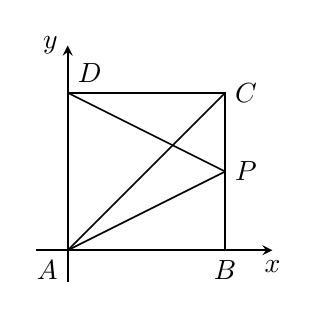
\begin{tikzpicture}[>=stealth,line width=0.6pt,font=\normalsize]
  \draw[->] (-0.4,0) -- (2.6,0) node[below] {$x$};
  \draw[->] (0,-0.4) -- (0,2.6) node[left] {$y$};
  
  \coordinate (A) at (0,0);
  \coordinate (B) at (2,0);
  \coordinate (C) at (2,2);
  \coordinate (D) at (0,2);
  \coordinate (P) at (2,1);

  \draw (A) -- (B) -- (C) -- (D) -- cycle;
  \draw (A) -- (C);
  \draw (A) -- (P);
  \draw (D) -- (P);

  \node[below left] at (A) {$A$};
  \node[below] at (B) {$B$};
  \node[right] at (C) {$C$};
  \node[above right] at (D) {$D$};
  \node[right] at (P) {$P$};
\end{tikzpicture}
